%\usepackage[T1]{fontenc}
%\usepackage[utf8]{inputenc}

%!TEX ROOT=../diploma-thesis.tex

\chapter{Verifikace a validace}\label{ch:verifikace}

V této kapitole si popíšeme, jaký způsobem byla provedena
verifikace naprogramovaných knihoven pomocí
jednotkových a integračních testů~\cite{luo2001software}
a také jejich nasazení při vývoji ukázkového systému.
Tím zároveň zvalidujeme koncept frameworku a shrneme výhody
a nevýhody jeho použití.

\section{Testování prototypů knihoven}

Prototypy knihoven, jejichž implementaci jsme popsali
v kapitole~\ref{ch:implementace}, byly také důkladně
otestovány pomocí sady jednotkových a integračních testů.

V rámci konceptu \textit{continous integration}~\cite{fowler2006continuous}
byl kód po celou dobu vývoje zasílán do centrálního repozitáře
a s pomocí nástroje Travis CI\footnote{https://travis-ci.org/}
bylo automaticky spouštěno jeho sestavení a otestování. Systém
zároveň okamžitě informoval vývojáře o jejich výsledcích. To
umožnilo v krátkém časovém horizontu identifikovat konkrétní změny
v kódu, které do programu vnesly chybu. Tím byla snížena
pravděpodobnost regrese a dlouhodobě se zvýšila celková kvalita kódu.

\subsection{Platforma Java}

\lstinputlisting[
caption={Příklad jednotkového testu knihovny pro jazyk Java s využitím nástroje JUnit 4},
label={lst:java-testing},
language=Java,
%frame=single
]
{code/test_example.java}

Prototyp knihovny pro platformu jazyka Java byl testován pomocí
nástroje JUnit~\cite{junit4}, který poskytuje versatilní platformu pro
jednotkové i integrační testování. Všechny testy byly spouštěny automaticky
při sestavování knihovny pomocí nástroje Maven~\cite{maven}.

Ve zdrojovém kódu~\ref{lst:java-testing}
můžeme vidět jednotkový test třídy \code{BusinessContextWeaver} ověřující,
že byly správně aplikovány post-conditions daného byznys kontextu, konkrétně
že bylo správně zakryto pole \code{email} objektu \code{user}. Anotace
\code{@Test} metody \code{test()} značí,
že metoda obsahuje \textit{test case} a framework JUnit zajistí, že bude spuštěna
a vyhodnocena. Statické metody třídy \code{Assert} ověří, zda uživateli zůstalo
vyplněno jméno, ale emailová adresa ne.


\subsection{Platforma Python}

\lstinputlisting[
caption={Příklad jednotkového testu knihovny pro jazyk Python s využitím nástroje Unittest},
label={lst:python-testing},
language=Python,
%frame=single
]
{code/test_example.py}

Prototyp knihovny pro platformu jazyka Python byl testován pomocí
nástroje \code{unittest}~\cite{pythonunittest}, inspirovaného nástrojem
JUnit. Ačkoliv jméno obou nástrojů nasvědčuje, že slouží zejména pro jednotkové testy,
lze je plně využít i pro integrační testy. Ve zdrojovém kódu~\ref{lst:python-testing} můžeme
vidět jednotkový test třídy \code{Identifier} se třemi metodami ověřujícími jeho
správnou funkcionalitu.

% TODO: popsat příklad

\subsection{Platforma Node.js}

Jelikož tendence ve světě moderního JavaScriptu je vytvářet knihovny s co nejmenším polem působnosti,
které jdou kombinovat do většího celku, byl prototyp knihovny pro platformu Node.js testován pomocí
kombinace několika nástrojů. Spouštění testů obstarává knihovna \textit{Mocha}~\cite{mocha}, zatímco
o ověřování samotné se stará knihovna \textit{Chai}~\cite{chai}. Zdrojový kód~\ref{lst:nodejs-testing}
znázorňuje použití knihoven k ověření správné funkcionality výrazu \code{IsNotNull}.

% TODO: popsat příklad

\lstinputlisting[
caption={Příklad jednotkového testu knihovny pro platformu Node.js s využitím nástroje Mocha a Chai},
label={lst:nodejs-testing},
language=JavaScript,
%frame=single
]
{code/test_example.js}

\section{Případová studie: e-commerce systém}

Abychom mohli navržený a implementovaný framework pro centrální správu
a automatickou distribuci byznys pravidel verifikovat v praxi a validovat
jeho myšlenku, bylo nutné ho nasadit při vývoji aplikace.
Pro tento účel vznikla v rámci této práce případová studie na fiktivním
ukázkovém e-commerce systému využívající architekturu orientovanou na služby.
Na tomto příkladě demonstrujeme schopnost frameworku poradit si s průřezovými
problémy v rámci SOA a také jeho schopnost plnit požadavky identifikované v
sekci~\ref{sec:implementation-requirements}.

\subsection{Use-cases}

Pro ukázkový systém bylo vymodelováno následujících třináct případů užití
(z anglického \textit{Use case} (UC)~\cite{bittner2002use}), jejich
přehled je v tabulce~\ref{tbl:use-cases}.

\begin{table}
    \centering
    \begin{tabular}{ l l }
        \hline
        \textbf{\#} & \textbf{Use-case} \\
        \hline \hline
        \textbf{UC01} & Nepřihlášený uživatel si může vytvořit zákaznícký účet \\
        \textbf{UC02} & Zákazník může prohlížet produkty \\
        \textbf{UC03} & Zákazník může vkládat produkty do košíku \\
        \textbf{UC04} & Zákazník může vytvořit objednávku \\
        \textbf{UC05} & Skladník si může prohlížet produkty \\
        \textbf{UC06} & Skladník může do systému zadávat nové produkty \\
        \textbf{UC07} & Skladník může upravovat u produktů stav skladových zásob \\
        \textbf{UC08} & Skladník si může zobrazovat objednávky \\
        \textbf{UC09} & Skladník může upravovat stav objednávek \\
        \textbf{UC10} & Administrátor si může prohlížet objednávky \\
        \textbf{UC11} & Administrátor může upravovat cenu produktů \\
        \textbf{UC12} & Administrátor může vytvářet uživatele (skladníky) \\
        \textbf{UC13} & Administrátor může mazat uživatele (skladníky i zákazníky) \\
        \hline
    \end{tabular}
    \caption{Přehled use-cases ukázkového e-commerce systému}
    \label{tbl:use-cases}
\end{table}

\subsection{Model systému}

Na obrázku~\ref{fig:example-model} můžeme vidět diagram tříd reprezentujících
kompletní doménový model ukázkového systému.

\begin{itemize}
    \item \textbf{\code{UserRole}} reprezentuje uživatelskou roli v systému.
    \item \textbf{\code{User}} je entita odpovídající uživateli, ať už zákazníkovi, či zaměstnanci.
    \item \textbf{\code{Product}} popisuje konkrétní produkt v nabídce společnosti a jeho nákupní a prodejní cenu.
    \item \textbf{\code{Order}} odpovídá objednávce, má vazbu na dodací a fakturační adresu a také na položky objednávky.
    \item \textbf{\code{OrderItem}} reprezentuje položku objednávky a uchovává údaje o počtu objednaných kusů produktu.
    \item \textbf{\code{Address}} je entita popisující dodací či fakturační adresu.
\end{itemize}

\begin{figure}
    \centering
    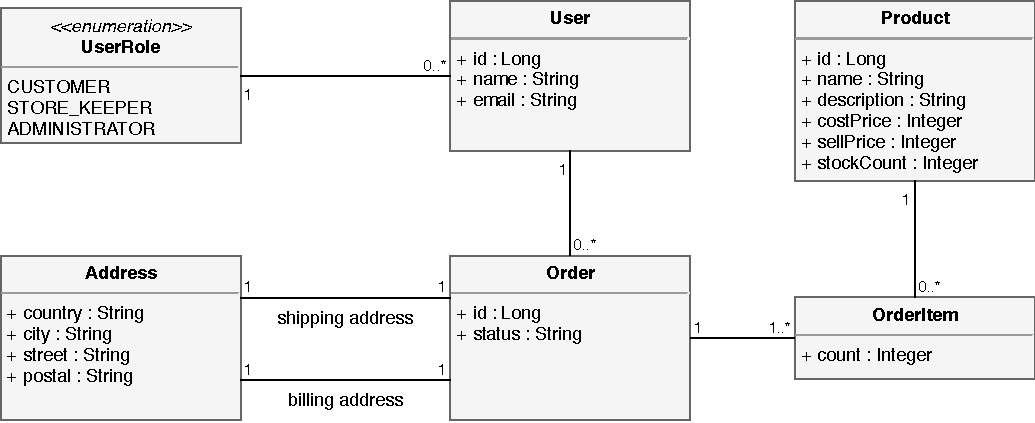
\includegraphics[keepaspectratio=true, width=0.9\linewidth]{figures/example-model.pdf}
    \caption{Diagram tříd modelu ukázkového e-commerce systému}
    \label{fig:example-model}
\end{figure}

Tento model je využíván v každé ze služeb. Nicméně, ne každá služba využije všechny jeho entity,
ale pouze jejich podmnožinu, kterou potřebuje ke svojí práci.

\subsection{Byznys kontexty a jejich pravidla}

V tabulce~\ref{tbl:business-rules} je výčet všech byznysových pravidel, která byla
vymodelována pro ukázkovou aplikaci. V tabulce kromě identifikátoru a popisu byznysového pravidla
vidíme, na které užitné případy se pravidlo aplikuje, a jaký je typ pravidla
(\textit{pre} pro precondition, \textit{post} pro post-condition).

\begin{table}
    \centering
    \begin{tabular}{ l l c r }
        \hline
        \textbf{\#} & \textbf{Use-cases} & \textbf{Pravidlo} & \textbf{Typ} \\ \hline \hline
        \textbf{BR01} & UC01 & Uživatel nesmí být přihlášený & pre \\ \hline
        \textbf{BR02} & UC02, UC03 & \makecell[c]{Uživatel nesmí zobrazovat ani manipulovat \\ s produkty, které nejsou aktivní} & post \\ \hline
        \textbf{BR03} & UC02 až UC04 & \makecell[c]{Uživatel nesmí u produktu vidět nákupní cenu, \\ pouze výslednou cenu} & post \\ \hline
        \textbf{BR04} & UC04 & \makecell[c]{Uživatel musí řádně vyplnit doručovací \\ adresu (č.p., ulice, město, PSČ, stát)} & pre \\ \hline
        \textbf{BR05} & UC04 & \makecell[c]{Uživatel musí řádně vyplnit fakturační \\ adresu (č.p., ulice, město, PSČ, stát)} & pre \\ \hline
        \textbf{BR06} & UC01, UC04 & Zákazník musí mít vyplněnou emailovou adresu & pre \\ \hline
        \textbf{BR07} & UC04 & Položky objednávky musí mít počet kusů větší než 0 & pre \\ \hline
        \textbf{BR08} & UC04 & \makecell[c]{Položky objednávky musí mít počet kusů menší, \\ než je aktuální stav skladových zásob produktu} & pre \\ \hline
        \textbf{BR09} & UC04 & \makecell[c]{Stát musí být v seznamu zemí, \\ do kterých firma doručuje} & pre \\ \hline
        \textbf{BR10} & UC04 & Zákazník musí být přihlášen & pre \\ \hline
        \textbf{BR11} & UC05 až UC09 & \makecell[c]{Skladník musí být do systému přihlášen \\ a mít roli "Skladník"} & pre \\ \hline
        \textbf{BR12} & UC05 & \makecell[c]{Skladník u produktu nesmí vidět nákupní cenu, \\ pouze výslednou cenu} & post \\ \hline
        \textbf{BR13} & UC06 & Produkt musí mít jméno s délkou >5 & pre \\ \hline
        \textbf{BR14} & UC07 & Stav zásob produktů musí být číslo větší nebo rovno 0 & pre \\ \hline
        \textbf{BR15} & UC08 & Skladník nesmí vidět celkový součet cen objednávek & post \\ \hline
        \textbf{BR16} & UC09 & \makecell[c]{Stav objednávky musí být pouze "přijato", \\ "expedováno" a "doručeno"} & pre \\ \hline
        \textbf{BR17} & UC10 až UC13 & \makecell[c]{Administrátor musí být do systému přihlášen \\ a mít roli "Administrátor"} & pre \\ \hline
        \textbf{BR18} & UC11 & \makecell[c]{Výsledná cena produktu musí být větší \\ než jeho nákupní cena} & pre \\ \hline
        \textbf{BR19} & UC12 & Skladník musí mít jméno delší než 2 znaky & pre \\ \hline
        \textbf{BR20} & UC12 & Skladník musí mít emailovou adresu v platném formátu & pre \\
        \hline
    \end{tabular}
    \caption{Přehled byznysových pravidel ukázkového e-commerce systému}
    \label{tbl:business-rules}
\end{table}

% TODO: seznam business contexts

Na obrázku~\ref{fig:example-system-context-hirearchy} můžeme vidět vizualizaci
hirearchie byznysových kontextů v ukázkovém systému, jejich vazbu na UC a také byznysová
pravidla, která se v kontextech aplikují.

\subsection{Služby}

Na obrázku~\ref{fig:example-system} můžeme vidět komponenty systému a jejich závislosti.
Pro ověření schopnosti podporovat více platforem byly pro implementaci systému využity
jazyky Java, Python a JavaScript v kombinaci s běhovým prostředím Node.js.

\begin{figure}
    \centering
    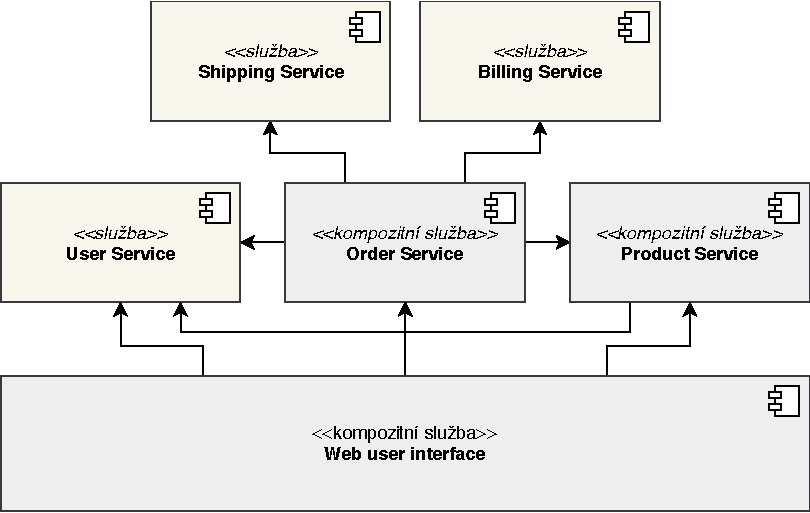
\includegraphics[keepaspectratio=true, width=0.8\linewidth]{figures/example-system.pdf}
    \caption{Diagram komponent ukázkového e-commerce systému}
    \label{fig:example-system}
\end{figure}

\paragraph{Service discovery}

Pro demonstrativní účely byly síťové adresy nastaveny přímo v kódu jednotlivých
služeb. Nicméně, navržený framework nevynucuje tento přístup, a tudíž by složitější
způsob \textit{service discovery} nebylo problém do systému integrovat.

\paragraph{Order service}

Kompozitní služba \textit{Order service} sloužící pro vytváření a správu objednávek
byla implementována v jazyce Java za použití framework Spring Boot~\cite{springboot}.

% TODO: jaké splňuje use-cases?

\paragraph{Product service}

Tato služba realizuje užitné scénáře spjaté s prohlížením a administrací nabízených
produktů a jejich skladových zásob. Služba byla implementována v jazyce Python.
Pro vytvoření REST API služby byl využit populární light-weight framework \textit{Flask}~\cite{flask}.
Ve zdrojovém kódu~\ref{lst:product-service-flask} můžeme vidět použití tohoto frameworku pro obsluhu
požadavku na výpis všech produktů.

% TODO: jaké splňuje use-cases?

\lstinputlisting[
caption={Ukázka využití frameworku Flask pro účely product service},
label={lst:product-service-flask},
language=Python,
%frame=single,
]
{code/product_service.py}

\paragraph{User service}

% TODO: jaké splňuje use-cases?

\paragraph{Nasazení systému pro centrální správu byznys kontextů}


\paragraph{Běhové prostředí služeb}
Pro jednoduché spuštění celého ukázkového systému byla využita technologie
Docker~\cite{merkel2014docker}, která umožňuje vytvořit virtuální běhové prostředí
pro aplikaci pomocí kontejnerizace využívající virtualizaci nad operačním systémem.
Uživatel si nadefinuje tzv. \textit{image}, který se skládá z jednotlivých vrstev.
Základní vrstvou je operační systém, dalšími mohou být jednotlivé knihovny instalované do systému.
Příklad definice image pomocí technologie Docker můžeme vidět ve zdrojovém
kódu~\ref{lst:docker-image}. Konkrétně se jedná o definici image, který
dědí od oficiálního image \code{library/node:9.11.1}~\cite{dockernodeimage} stavějícím nad operačním systémem \textit{Linux}~\cite{linux},
a přidává vrstvy s prototypem knihovny našeho frameworku pro platformu Node.js.

\lstinputlisting[
caption={Ukázka zápisu Docker image obsahující knihovnu pro platformu Node.js},
label={lst:docker-image},
language=Dockerfile,
%frame=single,
]
{code/dockerfile_nodejs.txt}

\paragraph{Spouštění služeb}
Pro samotné spuštění byla využita funkce \textit{Compose}, která umožňuje
definovat a spouštět více-kontejnerové aplikace. Ve zdrojovém kódu~\ref{lst:docker-compose}
můžeme vidět zápis Order service. Pro její image je použit \code{filipklimes-diploma/example-order-service}.
V sekci \code{ports} deklarujeme, že služba má mít z vnějšku přístupný port \code{5501}, na kterém poskytuje své
REST API, a port \code{5551}, nak terém poskytuje své gRPC API pro sdílené byzynsových kontextů. Order service je závislá
na Product, Billing, Shipping a User service, což explicitně specifikujeme v sekci \code{depends\_on},
aby Docker Compose mohl spustit služby ve správném pořadí. Nakonec pomocí \code{links} deklarujeme,
že pro kontejner, ve kterém Order Service poběží, mají být na síti přístupné služby \code{product}, \code{user},
\code{billing} a \code{shipping}. Vše je popsáno ve formátu YAML~\cite{ben2005yaml}, který je běžně využíván
pro konfigurační soubory, díky jeho snadné čitelnosti pro člověka a jednoduchému používání.

\lstinputlisting[
caption={Ukázka zápisu více-kontejnerové aplikace pro Docker Compose},
label={lst:docker-compose},
language=Yaml,
%frame=single,
]
{code/docker_compose.yml}

\section{Srovnání s konvenčním přístupem}

% TODO: bacha na to že teď je to v závěru, možná pak přesunout

\section{Shrnutí}

% TODO: shrnout
